\documentclass[12pt]{article}

\title{\vspace{-3em}PHYS 163a HW 2}
\author{Michael Cardiff}
\date{\today}

%% science symbols 
\usepackage{amsmath}
\usepackage{amssymb}
\usepackage{physics}
\usepackage{slashed}

%% general pretty stuff
\usepackage{bm}
\usepackage{enumitem}
\usepackage{float}
\usepackage{graphicx}
\usepackage[margin=1in]{geometry}
\usepackage[labelfont=bf]{caption}
\usepackage{siunitx}

% figures
\graphicspath{ {./figs/} }

\newcommand{\fig}[3]
{
  \begin{figure}[H]
    \centering
    \includegraphics[width=#1cm]{#2}
    \caption{#3}
  \end{figure}
}

\newcommand{\figref}[4]
{
  \begin{figure}[H]
    \centering
    \includegraphics[width=#1cm]{#2}
    \caption{#3}
    \label{#4}
  \end{figure}
}

\renewcommand{\L}{\mathcal{L}}
\newcommand{\D}{\partial}
\newcommand{\munu}{{\mu\nu}}
\newcommand{\sla}[1]{\slashed{#1}}

\begin{document}
\maketitle

\section{Poisson Distribution For Grades}
We can indicate that within the overall population of students, 10\% of them receive an A, that means in a population of 24 students, we expect $0.10\times24=2.4$ students to get an A, this will be $\lambda$ for our Poisson Distribution:
\begin{align*}
  P(X=k)=\eval{\frac{\lambda^k}{k!}e^{-\lambda}}_{\lambda=2.4}
\end{align*}
Plugging in $k=12$ gives us the probability of 12 students getting an A:
\begin{align*}
  P(X=12)=\frac{(2.4)^{12}}{12!}e^{-2.4}=\num{6.9e-6}
\end{align*}
Which is a $0.00069\%$ chance that 12 students get an A:
\begin{align}
  \boxed{P(X=12)=\num{6.9e-6}}
\end{align}
\section{Vegas Game}
We can make a table with all of the outcomes:
\begin{table}[H]
  \centering
  \begin{tabular}{c|c|c}
    Option & Outcome & Probability \\\hline
    1 & -2\$ & $p_1$\\
    2 & +0\$ & $p_2$\\
    3 & +4\$ & $p_3$
  \end{tabular}
  \caption{Possible Outcomes/Probabilities}
\end{table}
The various outcomes are $x_i$ and $p_i$ is $p(x_i)$ in short. We have two different constraints we need to enforce:
\begin{gather*}
  \sum_ip_i=1\\
  \sum_ix_ip_i=0
\end{gather*}
We can add these as the following Lagrange multipliers to our entropy:
\begin{align*}
  S_\alpha&=-\alpha\qty[\qty(\sum_{i=1}^3p_i)-1]\\
  S_\beta &=-\beta\qty[\qty(\sum_{i=1}^3x_ip_i)-0]
\end{align*}
And the total entropy is:
\begin{align*}
  S=-\qty[\sum_{i=1}^3p_i\ln p_i]-\alpha\qty[\qty(\sum_{i=1}^3p_i)-1]
  -\beta\qty[\qty(\sum_{i=1}^3x_ip_i)-0]
\end{align*}
To minimize entropy with respect to $p_i$ and $\alpha,\beta$, we need the gradient to be $0$:
\begin{align*}
  \grad_{\{p_i\},\alpha,\beta}S(\{p_i\},\alpha,\beta)=0
\end{align*}
Note that this odd looking gradient is:
\begin{align*}
  \grad_{\{p_i\},\alpha,\beta}=\qty(\qty{\pdv{p_i}},\pdv{\alpha},\pdv{\beta})
\end{align*}
That is, for this case:
\begin{align*}
  \grad_{\{p_i\},\alpha,\beta}=
  \qty(\pdv{p_1},\pdv{p_2},\pdv{p_3},\pdv{\alpha},\pdv{\beta})
\end{align*}
Taking the $\alpha$ and $\beta$ components first we get:
\begin{align*}
  \pdv{S}{\alpha}&=-\qty(p_1+p_2+p_3-1)=0\implies p_1+p_2+p_3=1\\
  \pdv{S}{\beta}&=-\qty(-2p_1+4p_3)=0\implies p_3=\frac{p_1}{2}
\end{align*}
We can use the second to get a bound of $p_2$ in terms of $p_1$, completely parameterizing our system:
\begin{align*}
  p_1+p_2+p_3=p_1+p_2+\frac{p_1}{2}=\frac32p_1+p_2=1\implies p_2=1-\frac32p_1
\end{align*}
Therefore the relationship between each of these is:
\begin{align*}
  (p_1,p_2,p_3)=\qty(p_1,1-\frac32p_1,\frac12p_1)
\end{align*}
Now we should rewrite the entropy in terms of this parameterization of solutions, knowing that it satisfies our constraints by construction, we have effectively eliminated $\alpha,\beta$:
\begin{align*}
  S(p_1)=-\sum_{i=1}^3p_i(p_1)\ln p_i(p_1)
\end{align*}
Where $p_i(p_1)$ is an element of the above vector:
\begin{align*}
  S(p_1)=-p_1\ln p_1-\qty(1-\frac32p_1)\ln(1-\frac32p_1)-\frac12p_1\ln\frac12p_1
\end{align*}
Differentiating with respect to $p_1$:
\begin{align*}
  \pdv{S(p_1)}{p_1}=\frac32\ln(1-\frac32p_1)-\frac32\ln(\frac{p_1}2)-\ln(p_1)
\end{align*}
This needs to be $0$, and since this is a transcendental equation I will solve it using numerical methods (a.k.a. Mathematica):
\begin{align*}
  \frac32\ln(1-\frac32p_1)-\frac32\ln(\frac{p_1}2)-\ln(p_1)=0\implies
  p_1=0.435977
\end{align*}
Thus giving the following probability distribution:
\begin{equation}
  \boxed{
    \begin{aligned}
      p_1&=0.435977\\
      p_2&=0.346035\\
      p_3&=0.217988
    \end{aligned}
  }
\end{equation}
\section{Dice Information Theory}
\subsection{Probability Distribution}
The unbiased probabilities require optimization of the entropy with the constraints that $\sum p_i=1$ and that $p_6=2p_1$. We know the other values $p_2...p_5$ should still all be equal like a normal dice. We can call this $p_0$ as it is an already optimized probability, so we need to optimize:
\begin{align*}
  S(p_1,p_o)=-p_1\ln p_1-2p_1\ln 2p_1-4p_o\ln(p_o)
\end{align*}
The probability of something else happening besides 1 or 6 is $p_o$, and we should be able to find it using the sum constraint:
\begin{align*}
  \sum_{i=1}^6p_i=3p_1+p_2+p_3+p_4+p_5=1
\end{align*}
If we all call them individually $p_o$:
\begin{align*}
  3p_1+p_2+p_3+p_4+p_5=1\implies3p_1+4p_o=1\implies p_o=\frac{1-3p_1}{4}
\end{align*}
Hence the entropy is:
\begin{align*}
  S(p_1)=-p_1\ln p_1-2p_1\ln 2p_1-(1-3p_1)\ln(\frac{1-3p_1}{4})
\end{align*}
The minimum is given by:
\begin{align*}
  \pdv{S}{p_1}&=-\ln p_1-2\ln 2p_1+3\ln(\frac{1-3p_1}{4})\\
  &=-\ln p_1-\ln((2p_1)^2)+\ln(\qty(\frac{1-3p_1}{4})^3)\\
  &=-\ln(2^2p_1^3)+\ln(\frac{(1-3p_1)^3}{2^6})\\
  &=\ln(\frac{(1-3p_1)^3}{2^8p_1^3})\\
  &=3\ln(\frac{1-3p_1}{2^{8/3}p_1})
\end{align*}
Solving for when this is $0$:
\begin{align*}
  3\ln(\frac{1-3p_1}{2^{8/3}p_1})&=0\\
  \frac{1-3p_1}{2^{8/3}p_1}&=1\\
  1-3p_1&=2^{8/3}p_1\\
  \qty(2^{8/3}+3)p_1&=1\\
  p_1&=\frac1{2^{8/3}+3}
\end{align*}
Then $p_1$ and $p_6$ are:
\begin{align*}
  p_1&=\frac1{2^{8/3}+3}\\
  p_6=2p_1&=\frac2{2^{8/3}+3}
\end{align*}
The remaining probabilities:
\begin{align*}
  p_2=p_3=p_4=p_5&=\frac{1-3p_1}4=
  \frac14\qty(\frac{2^{8/3}+3}{2^{8/3}+3}-\frac3{2^{8/3}+3})\\
  &=\frac{2^{8/3}/2^2}{2^{8/3}+3}\\
  &=\frac{2^{2/3}}{2^{8/3}+3}
\end{align*}
Hence the probability distribution is:
\begin{equation}
  \boxed{
    \begin{aligned}
      p_1&=\frac1{2^{8/3}+3}\\
      p_2=p_3=p_4=p_5&=\frac{2^{2/3}}{2^{8/3}+3}\\
      p_6&=\frac2{2^{8/3}+3}
    \end{aligned}
  }
\end{equation}

\subsection{Information Content}
The 'language' here is dice, with $M=6$, and the information content is:
\begin{align*}
  I&=\log_26+\sum_{i=1}^{6}p_i\log_2p_i\\
  &\approx 0.03
\end{align*}
The work from this:
\begin{center}
  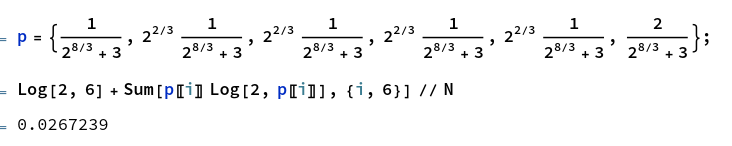
\includegraphics[width=15.0cm]{work.png}
\end{center}
Thus:
\begin{align}
  \boxed{I\approx 0.03\text{ bits}}
\end{align}
\section{Random Matrices}
\subsection{Characteristic Function of Each Element}
Each element has the same probability distribution in the interval $(-a,a)$, its even properly normalized, so the characteristic function $\tilde{p}(k)$ is:
\begin{align*}
  \tilde{p}_{ij}(k)&=\int_{-a}^a\frac{e^{-ikx}}{2a}\dd{x}\\
  &=\eval{\frac{e^{-ikx}}{-2ika}}_{-a}^a\\
  &=\frac{e^{ika}-e^{-ika}}{2ika}
\end{align*}
This can be reduced to $\sin(ka)$ using euler's identity:
\begin{align}
  \boxed{\tilde{p}_{ij}(k)=\frac{\sin ka}{ka}}
\end{align}
\subsection{Characteristic Function for the Trace}
Note that the trace is found by adding together diagonal elements of of a matrix, and since this matrix is $N$ by $N$, we are adding $N$ elements to get the trace.

If we want to find the characteristic function for a random variable that can be described as the sum of other random variables where we already know the characteristic functions, we can simply take the product of all the ones we know to get the one we dont. Hence, since we have $N$ of the same function, we get that:
\begin{align}
  \boxed{\tilde{p}_{Trace}=\qty(\frac{\sin ka}{ka})^N}
\end{align}
\subsection{Central Limit Theorem}
The central limit theorem states that for a large number of summed independent random variables, it is approximately normally distributed. This means that the cumulants of the sum is just the sum of the individual cumulants. This means the leading order cumulants are:
\begin{equation}
  \boxed{
    \begin{aligned}
      \ev{Trace}_c=N\ev{M_{ij}}&=0\\
      \ev{Trace^2}_c=N\ev{M_{ij}^2}=N\int_{-a}^a\frac{x^2}{2a}\dd{x}&=
      \frac{Na^2}{3}
    \end{aligned}
  }
\end{equation}
\subsection{Variance of Wigner Semicircle Rule}
For the following probability distribution we want to find the variance:
\begin{align*}
  \sigma^2_\lambda=\ev{\lambda^2}-\ev{\lambda}^2
\end{align*}
The first expectation value is:
\begin{align*}
  \ev{\lambda}&=\frac2{\pi\lambda_0}\int_{-\lambda_0}^{\lambda_0}\lambda
  \sqrt{1-\frac{\lambda^2}{\lambda_0^2}}\dd{\lambda}\\
  x&=\frac\lambda{\lambda_0}\qquad \dd{x}=\dd{\lambda}/\lambda_0\\
  &=\frac{2\lambda_0}{\pi}\int_{-1}^1x\sqrt{1-x^2}\dd{x}\\
  u&=1-x^2 \qquad \dd{u}=-2x\dd{x}\\
  &=-\frac{\lambda_0}\pi\int_0^0\sqrt{u}\dd{u}=\boxed{0}
\end{align*}
The second:
\begin{align*}
  \ev{\lambda^2}&=\frac2{\pi\lambda_0}\int_{-\lambda_0}^{\lambda_0}\lambda^2
  \sqrt{1-\frac{\lambda^2}{\lambda_0^2}}\dd{\lambda}\\
  x&=\frac\lambda{\lambda_0} \qquad \dd{x}=\dd{\lambda}/\lambda_0\\
  &=\frac{2\lambda_0^2}\pi\int_{-1}^1x^2\sqrt{1-x^2}\dd{x}\\
  x&=\sin\theta\qquad\dd{x}=\cos\theta\dd{\theta}\\
  &=\frac{2\lambda_0^2}\pi\int_{-\pi/2}^{\pi/2}\sin^2\theta\cos^2\theta\dd{\theta}
\end{align*}
This is a standard integral we can put in mathematica:
\begin{align*}
  \frac{2\lambda_0^2}\pi\int_{-\pi/2}^{\pi/2}\sin^2\theta\cos^2\theta\dd{\theta}
  &=\frac{\lambda_0^2}{4}
\end{align*}
Hence the variance is just this term:
\begin{align}
  \boxed{\sigma^2_\lambda=\frac{\lambda_0^2}{4}}
\end{align}
\subsection{Independent Eigenvalues?}
The eigenvalues are related to the trace by a sum:
\begin{align*}
  Trace=\sum_{i}\lambda_i
\end{align*}
So the expectation of the trace squared is going to be:
\begin{align*}
  \ev{Trace^2}=\sum_i\ev{\lambda_i^2}+\sum_{i\neq j}\ev{\lambda_i\lambda_j}
\end{align*}
We already have a form for the expectation of the trace squared via the central limit theorem, and we just calculated the expectation of $\lambda_i^2$, so its sum will be $N$ times that. However:
\begin{align*}
  \ev{Trace^2}-\sum_i\ev{\lambda_i^2}=\frac{Na^2}{3}-\frac{N^2a^2}{3}
\end{align*}
In order for the eigenvalues to be independent, the cross correlations must be $0$, which this is not!
\section{Water Weeds}
Each day will have a different, yet equally distributed random increase of the number density, meaning we can write the number density as a function of number of days $N>0$:
\begin{align*}
  n(N)=n_0\prod_{i=1}^N(1+\Delta_i)
\end{align*}
This product for large $n$ will contain at the very least the sum of all of the individual $\Delta_i$ as well as mixed products between all of them. And since the value of $\Delta$ will always be small, so will mixed products such as $\Delta_i\Delta_j$, so we can ignore them. According to the central limit theorem, since we have such a large sum over independent variables, the sum should be Normally Distributed, with mean $N\mu_{\Delta}=0$ and standard deviation $N\sigma_\Delta$.
\end{document}